% ======================================================================
\section{Sparse, clustered, and spatially localized representations}
\label{sec:local}
% ======================================================================

A global linear basis must represent every state as a superposition of the
same $r$ modes, each supported on the whole domain. The methods in this section
relax one of these two features. Sparse and clustered representations let the
set of active modes depend on the state. Spatially localized representations
restrict the support of each basis function to a subdomain. The resulting
representations are piecewise linear in state space or in physical space, and
therefore nonlinear or multi-scale overall. They keep much of the transparency,
cost, and robustness of linear methods.

\subsection{Sparse coding and dictionary learning}

Sparse coding represents each state as a combination of a few atoms from an
overcomplete dictionary $\bm{D}\in\R^{N\times K}$ with $K>N$ or $K>r$,
\begin{equation}
  \min_{\bm{D},\{\bm{s}_k\}}\;\sum_{k}\|\bm{x}_k-\bm{D}\bm{s}_k\|_2^2+\lambda\|\bm{s}_k\|_1,
\end{equation}
so that different states can activate different subsets of atoms.
Dictionaries learned from natural images reproduce the localized, oriented
receptive fields of the visual cortex \parencite{olshausen1996}. K-SVD is a
widely used algorithm for learning them \parencite{aharon2006ksvd}.
\textcite{deshmukh2016sparse} introduced sparse coding for basis identification
in fluid ROMs. Unlike POD, which truncates to the dominant energetic modes,
sparse coding seeks a compact representation spanning \emph{all} scales of the
data, and Galerkin models built on sparse modes of a lid-driven cavity flow were
substantially more predictive than POD--Galerkin models.
\textcite{deshmukh2018energy} traced this improvement to energy balance.
Multi-scale content in the retained modes lets the ROM balance production and
dissipation of energy, which a basis made only of large, energetic structures
cannot. Sparsity is also the foundation of compressed sensing
\parencite{candes2006robust,donoho2006cs}, which in fluids underlies sparse
sensor placement \parencite{manohar2018sensor} and flow reconstruction by
sparse representation in a library of training snapshots
\parencite{callaham2019robust}.

\subsection{Clustered and local bases in state, parameter, and time}

A second way to adapt the representation to the state is to partition the data
set and assign a separate low-dimensional description to each part.
\emph{Cluster-based reduced-order modeling} \parencite{kaiser2014cluster}
partitions snapshots into a small number of clusters by $k$-means, represents
each by its centroid, and models the dynamics as a Markov chain of transitions
between clusters, generalizing the Ulam--Galerkin approximation of the
Perron--Frobenius operator. \emph{Local reduced-order bases}
\parencite{amsallem2012local} cluster the solution space and build a separate
POD basis for each cluster, switching bases online as the state moves between
regions. They are aimed at problems with distinct physical regimes, parameter
variations, or moving fronts. Related ideas include local discrete empirical
interpolation \parencite{peherstorfer2014ldeim} and interpolation of bases
between parameter values on the Grassmann manifold
\parencite{amsallem2008grassmann}. These methods approximate a curved manifold
by a patchwork of tangent-like subspaces, a strategy mirrored in locally linear
embedding (\cref{sec:manifold}) and in the local linear decoder used by
\textcite{loiseau2018sparse}.

\subsection{Spatial localization and domain decomposition}

Localization in \emph{physical} space follows from a simple observation.
Correlations in turbulent flows decay with separation, so a structure in one
region carries little information about another. A global mode that captures a
structure in one region wastes degrees of freedom elsewhere, whereas a local
basis spends them only where needed and can be reused wherever similar
structures appear. Wavelet decompositions, which are localized in both
space and scale, were an early expression of this idea in turbulence analysis
\parencite{farge1992wavelet}. The idea has a long history in both reduced-order
modeling and numerical analysis.

In reduced-order modeling, \textcite{lucia2001thesis,lucia2003moving} treated the region swept by
a moving shock separately from the rest of a POD-based model, isolating the
feature that a global basis represents worst. The reduced basis element method
\parencite{maday2002rbe} and the static-condensation reduced basis element
method \parencite{huynh2013scrbe} build reduced bases for components or
subdomains and couple them across interfaces. Domain-decomposition strategies
have been developed for POD-based models of the incompressible Navier--Stokes
equations \parencite{baiges2013dd} and for reduced-basis methods in networks
and complex geometries \parencite{iapichino2016dd}. For extreme-scale problems,
where even storing global snapshots is prohibitive, domain-decomposition
least-squares Petrov--Galerkin (DD-LSPG) builds subdomain bases and couples
them through the governing equations \parencite{hoang2021ddlspg}.
\textcite{diaz2024ddnm} extended this approach to nonlinear manifolds, training
a separate shallow sparse autoencoder on each subdomain. The subdomain models
have fewer parameters, need smaller training sets, and can be trained in
parallel.

In numerical analysis, the partition-of-unity finite element method
\parencite{melenk1996pum} and the generalized finite element method (GFEM)
\parencite{babuska2004gfem} showed how to embed arbitrary local approximation
spaces into a conforming global approximation. Let $\{N_i\}$ be finite element
shape functions forming a partition of unity, $\sum_i N_i\equiv 1$, each
supported on the patch $\omega_i$ of elements sharing node $i$. Let
$\{\psi_{i,k}\}$ be any functions that approximate the solution well on
$\omega_i$. Then
\begin{equation}
  u(\bm{x})\approx\sum_{i}N_i(\bm{x})\Bigl[a_i+\sum_{k=1}^{m}b_{ik}\,\psi_{i,k}(\bm{x})\Bigr]
  \label{eq:gfem}
\end{equation}
inherits the local approximation quality of the enrichments $\psi_{i,k}$, while
the multiplication by $N_i$ keeps every basis function compactly supported and,
for continuous $N_i$ and $\psi_{i,k}$, globally $C^{0}$
\parencite{melenk1996pum}. \textcite{babuska2011optimal} characterized optimal
local approximation spaces for GFEM in multi-scale problems;
\textcite{smetana2016optimal} did the same for component-based static
condensation. The multiscale finite element method
\parencite{hou1997msfem} and its generalized variant
\parencite{efendiev2013gmsfem} construct local basis functions from local
solutions or local snapshot spaces. This is the same idea of numerically
computed, locally supported bases, derived from the operator instead of from
data.

\subsection{Data-informed local subspaces}
\label{sec:dls}

The Data-informed Local Subspace (DLS) method of \textcite{deshmukh2020dls}
brings the GFEM construction \eqref{eq:gfem} to data-driven representation of
turbulent flows. The enrichment functions are learned from snapshot data rather
than derived from the governing operator. The construction has four steps,
illustrated in one dimension in \cref{fig:dls_schematic}.
\begin{enumerate}[leftmargin=2.2em,itemsep=2pt]
  \item \emph{Coarse mesh and partition of unity.} A coarse mesh of linear (in
  two dimensions, bilinear) finite elements is laid over the data grid with
  nodes every $n_{\mathrm{skip}}$ grid points; its shape functions $N_i$ form
  a partition of unity (\cref{fig:dls_schematic}a).
  \item \emph{Local POD modes.} Patches of $(2n_{\mathrm{skip}}+1)^{d}$ grid
  points are sampled at random locations from the training snapshot(s). The
  mean of each patch is removed, and the patches are decomposed by POD
  (\cref{fig:dls_schematic}b). The leading $m$ local modes $\psi_k$ are shared
  by all nodes: the mode used at node $i$ is $\psi_k(\bm{x}-\bm{x}_i)$,
  centered on the node, so that its $(2n_{\mathrm{skip}}+1)^{d}$ footprint
  exactly covers the support $\omega_i$ of $N_i$.
  \item \emph{GFEM enrichment.} The local modes are multiplied by the shape
  functions, and the products $N_i(\bm{x})\,\psi_k(\bm{x}-\bm{x}_i)$ are used,
  together with the standard $N_i$, as the basis functions of \eqref{eq:gfem}
  (\cref{fig:dls_schematic}c). Each enrichment vanishes on the boundary of
  $\omega_i$, so the assembled representation is $C^{0}$-continuous across
  element boundaries. The local POD modes are thus not used directly as a
  block-wise basis: they enter only through the enriched GFEM space.
  \item \emph{Global projection.} The $(m+1)$ coefficients per node and field
  variable are obtained by $L^2$ projection onto the enriched space. The global
  mass matrix $\bm{M}$ is assembled from element matrices, and the load vector
  $\bm{L}$ from element-wise inner products with the data, giving
  $\bm{M}\bm{c}=\bm{L}$. On a uniform mesh with shared local modes all
  element mass matrices are identical, so $\bm{M}$ is sparse and is factorized
  once (\cref{fig:dls_schematic}d).
\end{enumerate}
The latent vector $\bm{c}$ has dimension $r=d_v\,n_{\mathrm{nodes}}\,(m+1)$
for $d_v$ field variables. Only the $m$ local modes of size
$(2n_{\mathrm{skip}}+1)^{d}$ per variable need to be stored in addition to the
coefficients. Following \textcite{deshmukh2020dls}, the compression ratio for
$T$ snapshots of an $M$-dimensional field in $d$ spatial dimensions (with $d$
velocity components) is
\begin{equation}
  \mathrm{CR}=\frac{M\,T}{d\,T\,n_{\mathrm{nodes}}(m+1)+d\,m\,(2n_{\mathrm{skip}}+1)^{d}}.
\end{equation}
Encoder and decoder are both linear, sparse, and local. The encoder is a
sparse linear solve and the decoder an element-wise sum.

Several properties make DLS attractive as a representation for learning.
(i) \emph{Data efficiency (P4).} Because patches are sampled \emph{within}
snapshots, a single snapshot provides thousands of training samples for the
local modes. \textcite{deshmukh2020dls} reported that, relative to global POD,
the GFEM approach increases reconstruction efficiency for a three-dimensional
cylinder flow at $\mathrm{Re}=10^{5}$ and for lid-driven cavity flows over a
range of Reynolds numbers, while substantially reducing the amount of training
data required. (ii) \emph{Multi-scale resolution (P1).} The coarse element size
sets the scale resolved by the standard FE part, and the local modes add
sub-element structure, so resolution is controlled locally rather than by
global energy ranking. (iii) \emph{Scalability (P5).} Encoding and decoding
are sparse operations whose cost grows linearly with $N$, and the basis is
independent of the number of snapshots. (iv) \emph{Structured latent space.}
The coefficients are attached to mesh nodes, so the latent state is itself a
coarse spatial field. Sequence models can therefore operate on it globally or
as spatially local tokens, analogous to the patch tokens of vision transformers
\parencite{dosovitskiy2021vit} or the local neural fields of AROMA
\parencite{serrano2024aroma}. The price is a larger latent dimension than a
global basis needs when the flow is dominated by a few coherent structures.

\textcite{morton2026scitech} used DLS latent spaces with transformer forecasting
for two-dimensional lid-driven cavity flow at $\mathrm{Re}=15{,}000$ and
$30{,}000$. They found that the DLS-based model reasonably reproduced the flow
dynamics and turbulence statistics at both Reynolds numbers, whereas models
trained on a POD latent space performed poorly. A related precedent for
exploiting locality in the \emph{dynamics} model is the parallel reservoir
computing approach of \textcite{pathak2018reservoir}, in which many small
reservoirs each forecast a local region of a large spatiotemporally chaotic
system.

\paragraph{A computed comparison.}
\Cref{fig:dls_compare,fig:dls_recon} compare global POD and DLS on held-out
snapshots of the $\mathrm{Re}=15{,}000$ cavity flow of \cref{fig:ldc_pod}.
DLS bases use local modes from a single training snapshot, while the POD basis
uses 2000 snapshots. Three observations follow. First,
at equal latent dimension global POD is far more compact for this flow
(\cref{fig:dls_compare}a). Its held-out error falls to 0.33\% with about 150
modes, beyond which the remaining modes carry negligible energy. DLS needs
roughly $10^{4}$ coefficients for 1\% error ($49^2$ patches, $m=10$) and
$2.6\times10^{4}$ for 0.45\% ($19^2$, $m=3$). At a budget of 1936
coefficients, DLS errors are 11--13\%, and the vorticity reconstructions show
element-scale artifacts (\cref{fig:dls_recon}). This is the expected outcome
for a flow whose fluctuation energy is 90\% contained in a single pair of
global modes (\cref{fig:ldc_pod}). Second, the comparison reverses when the
amount of training data is considered (\cref{fig:dls_compare}b). A POD basis
built from the first 512 snapshots has a held-out error of 8.3\%, and one
built from 1000 snapshots 1.8\%, whereas DLS bases whose local modes come from
a \emph{single} snapshot reach 1.0\% ($49^2$, $m=10$) and 0.45\% ($19^2$,
$m=3$). DLS accuracy is set by local resolution ($n_{\mathrm{skip}}$ and $m$),
not by how much of the flow's temporal variability the training record
happens to contain. Third, the singular values of small local patches decay
faster than those of the global snapshots (\cref{fig:dls_compare}c), which is
the local redundancy that the enrichment exploits. The example thus
illustrates the trade-off discussed in \cref{sec:assessment}. Global bases are
most compact for globally simple flows once enough data are available. Local
bases are data-efficient and scale with local rather than global complexity,
which matters most for broadband, multi-scale flows and for large domains
where long training records are unaffordable. Compactness of reconstruction
is also not the same as suitability for forecasting (\cref{sec:goodlatent}):
for this same cavity flow, \textcite{morton2026scitech} found transformer
forecasts on DLS latent spaces to be markedly better than on a POD latent
space.

\begin{figure}[tbp]
  \centering
  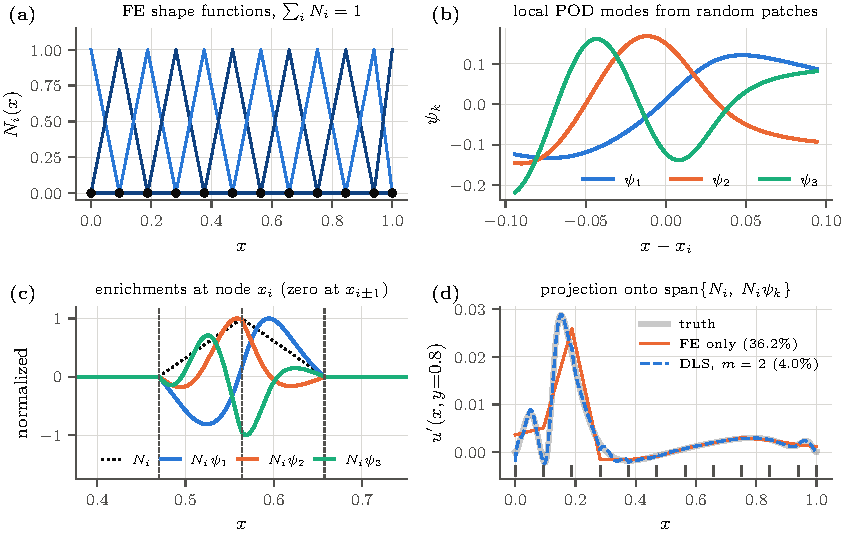
\includegraphics[width=\textwidth]{figs/dls_schematic.pdf}
  \caption{The DLS/GFEM construction in one dimension, applied to a horizontal
  line cut ($y=0.8$) of the fluctuating velocity in the $\mathrm{Re}=15{,}000$
  cavity. (a)~Linear finite element shape functions on a coarse mesh (nodes
  every $n_{\mathrm{skip}}=48$ grid points) form a partition of unity.
  (b)~Leading local POD modes of randomly sampled, mean-removed patches of
  $2n_{\mathrm{skip}}+1$ points. (c)~Enrichment functions
  $N_i(x)\,\psi_k(x-x_i)$ at one node: each is supported on the two elements
  adjacent to $x_i$ and vanishes at $x_{i\pm1}$, which guarantees
  $C^{0}$ continuity of the assembled field. (d)~$L^2$ projection of the signal
  onto the standard FE space alone and onto the enriched space with $m=2$ local
  modes; relative errors in parentheses.}
  \label{fig:dls_schematic}
\end{figure}


\begin{figure}[tbp]
  \centering
  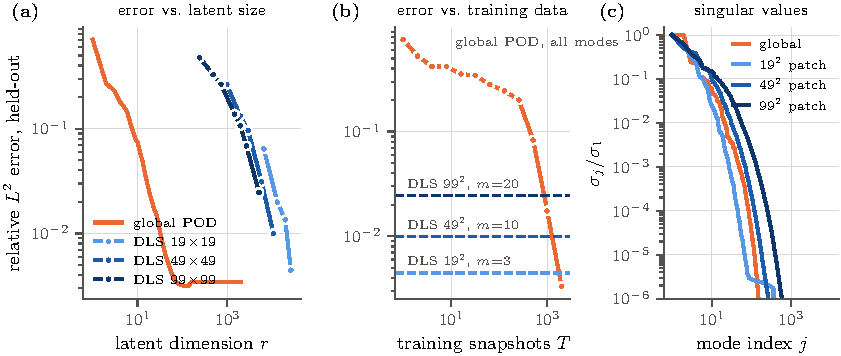
\includegraphics[width=\textwidth]{figs/ldc_local_global.pdf}
  \caption{Global POD versus DLS for the $\mathrm{Re}=15{,}000$ lid-driven cavity.
  (a)~Relative $L^2$ error of the fluctuating velocity on 90 held-out snapshots
  (separated in time from the training window) versus latent dimension. POD
  uses 2000 training snapshots; DLS uses local modes from a single training
  snapshot, with patch sizes $19^2$, $49^2$, and $99^2$ and
  $m$ local modes per node (markers, increasing $m$ from left).
  (b)~Error of global POD, keeping all non-negligible modes, when built from
  the first $T$ training snapshots. Dashed lines give the DLS errors of
  panel~(a) for the largest $m$ of each patch size, obtained from one snapshot.
  (c)~Normalized singular values of the global snapshot matrix and of the
  random local patches used to build the DLS modes. Errors are evaluated on
  the $491\times491$ region covered by all DLS meshes.}
  \label{fig:dls_compare}
\end{figure}

\begin{figure}[tbp]
  \centering
  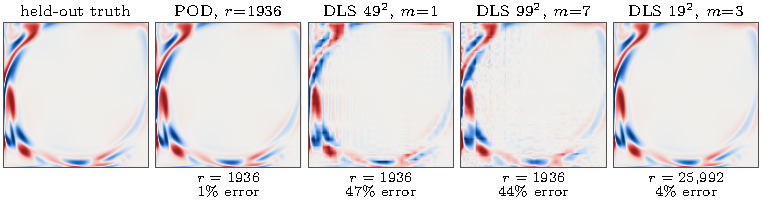
\includegraphics[width=\textwidth]{figs/ldc_local_recon.pdf}
  \caption{Fluctuating vorticity of a held-out cavity snapshot and its
  reconstructions. The middle three panels use the same number of latent
  coefficients ($r=1936$; for POD this includes all $\approx150$ modes with
  non-negligible energy). The right panel shows DLS with $19^2$ patches and
  $m=3$ ($r=25{,}992$). Percentages are relative $L^2$ errors of the
  vorticity, which weights small scales more heavily than the velocity errors
  of \cref{fig:dls_compare}.}
  \label{fig:dls_recon}
\end{figure}
